\section{Contextual Analysis}

	\subsection{Scope rules}
	These are the rules that defines how the identifiers must be read, and where to declare them - also known as identification.
	
	
	The WAR language has a nested block-structure which means we may have more scope levels. Scope rules may be defined in levels, such that a declaration in the outermost block is at scope level 1, however, since the language has no declaration of variables, only constants, it works the same way. If you declare the $Size$ of a regiment at scope level 1, you can use $Size$ in all the higher scope levels. Declarations inside a block are referred to as being local in that block.
		\newpage

	By using a nested block structure we follow some basic scope rules:
	\begin{wrapfigure}{r}{0.5\textwidth}
		\begin{center}
			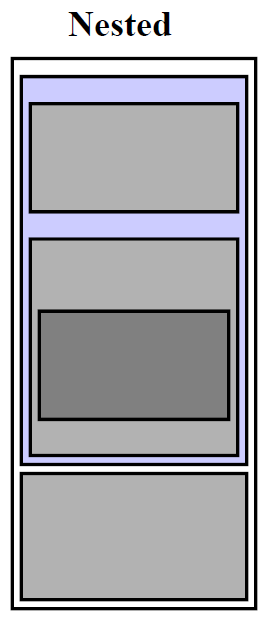
\includegraphics[scale=1]{rapport/5/figures/nested_block_structure}
		\end{center}	
		\caption{Illustration of the nested block structure}
		\label{nested_block_structure}
	\end{wrapfigure}


	%INCLUDE BIBLIOGRAPHY!!!	
	\begin{itemize}
	\item No identifier may be declared more than once within the same block (at the same level) %SPO
	\item For any applied occurrence there must be a corresponding occurrence, either within the same block or block which is higher up in the nesting. %SPO
	%INCLUDE BIBL...
	\end{itemize}
	
	
	Referring to figure \ref{nested_block_structure} which demonstrates the functioning of a nested block structure visually. Initially we consider how the nested block structure works in general and later an example of how the nested block structure works in the WAR programming language.
	
	One can have as many and as few blocks as needed, and every sub-block of an existing block, can use all the variables that have been declared in blocks over itself. 
	
	
	%Her kommer noget kode af vores egen for at beskrive hvordan nested block structure virker hos os.
		
	 
	
	

\newpage	

	
	
	
%Page 142 i Brown!! :D